\documentclass{article}

\usepackage[english]{babel}     %testi autogenerati italiano
\usepackage{graphicx}           %per importare immagini
\usepackage{geometry}           %per gestire margini e spostamenti
\usepackage{amsmath}
\usepackage{minted}
\usepackage{xcolor}
\usepackage[export]{adjustbox}
\usepackage[raggedright]{titlesec}
\geometry {
    top=20mm,
    bmargin=20mm,
}
\usepackage{array}              %per colonne di width fissata
\usepackage{subcaption}         %tabelle divise
\usepackage{hyperref}           %links
\hypersetup{
    colorlinks=true,
    linkcolor=black,
    urlcolor=blue
}
%\usepackage[bottom]{footmisc}   %footnotes fissate a piè pagina
\usepackage{booktabs}           %per tabitem in tabular
\newcommand{\tabitem}{~~\llap{\textbullet}~~}
\renewcommand*{\thefootnote}{[\arabic{footnote}]}

\begin{document}

\setlength\parindent{0pt} %noindent automatico
\setlength\parskip{1em}

\begin{titlepage}
	\centering
	\hrule
	
	\vspace{6,5cm}
	{\Huge \textbf{IoT Project: Keep your distance\\
		2020/21}\\}
		
		\vspace{0,5cm}
		\large {Prof. Cesana Matteo}
		
		\vspace{2,5cm}
		{
			\large
			\begin{tabular}{c c}
				Shalby Hazem Hesham Yousef & (Personal Code: 10596243) \\
			\end{tabular}
			
		}
		\vspace{5cm}
		\vspace{0,5cm}
		
		\centering\hspace{0,2cm}
\includegraphics[scale=0.6]{./logo.png}
		\vspace{0,5cm}
		\hrule
		
		\end{titlepage}
		
		\pagebreak
		
		\pagebreak
		
		\section{Structure description} %1
		\begin{figure}[h!]
         \begin{center}
        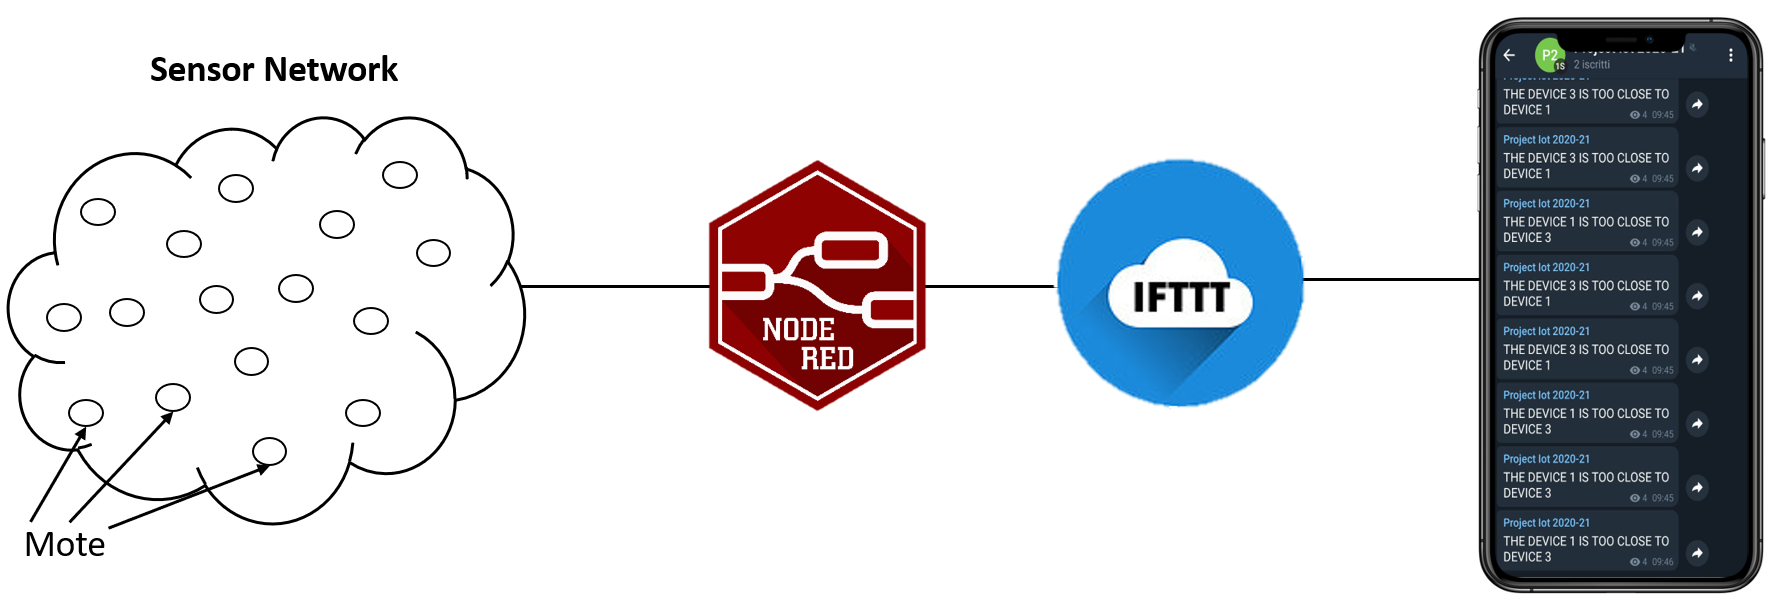
\includegraphics[width=1\textwidth]{./general_schema.png}            
        \end{center}
        \caption{General project schema}
        \label{fig:schema}
        \end{figure}
        The software purpose is to detect and alert the user when two people (motes) are close to each other.\footnote{two people/motes are close to each other when they remain close for at least 5 seconds (10 message)}.
The software structure, as in the Figure \ref{fig:schema}, could be split in three main parts:
\begin{itemize}
    \item The sensor network
    \item Node red
    \item IFTTT\footnote{IFTTT is a service to create conditional statements, and it’s an easy way to send notifications to your smartphone}
\end{itemize}
In the sensor network each mote broadcasts its presence every 500ms with a message containing its ID and a counter, which is incremented every time a message is sent. If a motes receives 10 consecutive messages from the same mote it triggers an alarm.\\
The alarm triggered by a mote is captured by node red via socket and then a web req to the IFTTT service is done.\\
The last component of the software (IFTTT) simply sends a message to the user using  a telegram channel. 
\subsection{THE SENSOR NETWORK} %1.1
Per se the motes code is very simple except for the part that triggers the alarm when 10 consecutive messages are received. To recognize/sense the event described before the developed code use two arrays:
\begin{itemize}
    \item \texttt{last\_msg\_count}    
    \item \texttt{cons\_msg\_count}
\end{itemize}
The first array (\texttt{last\_msg\_count}) save the last message count received from the other motes and it’s updated each time a new message is received, while the second one (\texttt{cons\_msg\_count}) take trace of the number of consecutive message received and it’s managed using the following rule.
\\
\[
\begin{cases}
    \texttt{cons\_msg\_count[rcm->id] = 1}   & \texttt{if last\_msg\_count[rcm->id] +1 < rcm->counter} \\
    \texttt{cons\_msg\_count[rcm->id]+= 1}  & \texttt{if last\_msg\_count[rcm->id] +1 == rcm->counter} \\
    \texttt{cons\_msg\_count[rcm->id] = 0}  & \texttt{if cons\_msg\_count[rcm->id]==10}
\end{cases}
\]
Note that:
\begin{itemize}
    \item In the previews rule \texttt{rcm} is the received message.
    \item If the last rule is rule is verified an alarm is triggered and the counter of the consecutive messages of the corresponding motes is reset.
    \item Both the array keep the information about each mote in the position corresponding to the mote ID (for example: in the mote with ID.2 arrays, information about mote 3 are saved in  the pos 3 of the two array)\footnote{The algorithm is described with arrays with index that starts from 1 but in the implementation the arrays starts from 0}
\end{itemize}
Another fact that is noteworthy is how the mote trigger an alarm. it's done by simply printing a JSON string containing the information about the two motes that produced the alarm. The following is an example of an alarm triggered because mote 3 and mote 4 were too close to each other.
\begin{minted}{json}
{
  "ALARM": {
    "id_first_mote": 3,
    "id_second_mote": 4
  }
}
\end{minted}



\subsection{THE NODE RED}
The node red part simply sends an http request, once it captures an alarm.\\
The node-red part could be divided into three parts:
\begin{itemize}
    \item Reception of messages: done via socket, one foreach mote.
    \item Parsing of messages: since motes send JSON strings as described before, this part of the code simply parse the received strings.
    \item Sending results: sending an HTTP request to the IFTTT service.
\end{itemize}
Noteworthy is the fact that, if two motes are too close to each other, two alarms are triggered but since the user in the simulation is only one, node red drops one of the two alarm (the one triggered by the mote with smallest id). The last rule is added only to enable a better understanding of the simulation part.
\subsection{IFTTT}
Once an HTTP request is received simply send a message to a public telegram channel \footnote{the link to join the telegram channel is the following: \href{https://t.me/iot_project_shalby}{Telegram Channel}}

\section{SIMULATION}

The simulation is done using 5 motes but could be extended to N mote, where N is a parameter in the code running on the node (by default is set to 10).\\
The simulation was used to test the behavior of the system under a lot of circumstances.
The simplest simulation is done by approaching and moving away two motes from each other to see their behavior.\\
Then a lot of simulation could be done extending the approach from two mote to multiple motes, and in particular four main simulation are noteworthy:
\begin{itemize}
    \item A mote crossing an aisle created by the other motes
    \item Motes that are all collapsed in one point moving away
    \item Motes not close to each other that are going to the same point
    \item A mote going from one side to the other of a room, crossing other nodes in its path (this similar to the first one but the other motes are sparsed)
\end{itemize}



\begin{figure}[h]
    \centering
    \begin{minipage}[c]{.3\linewidth}
        \centering
        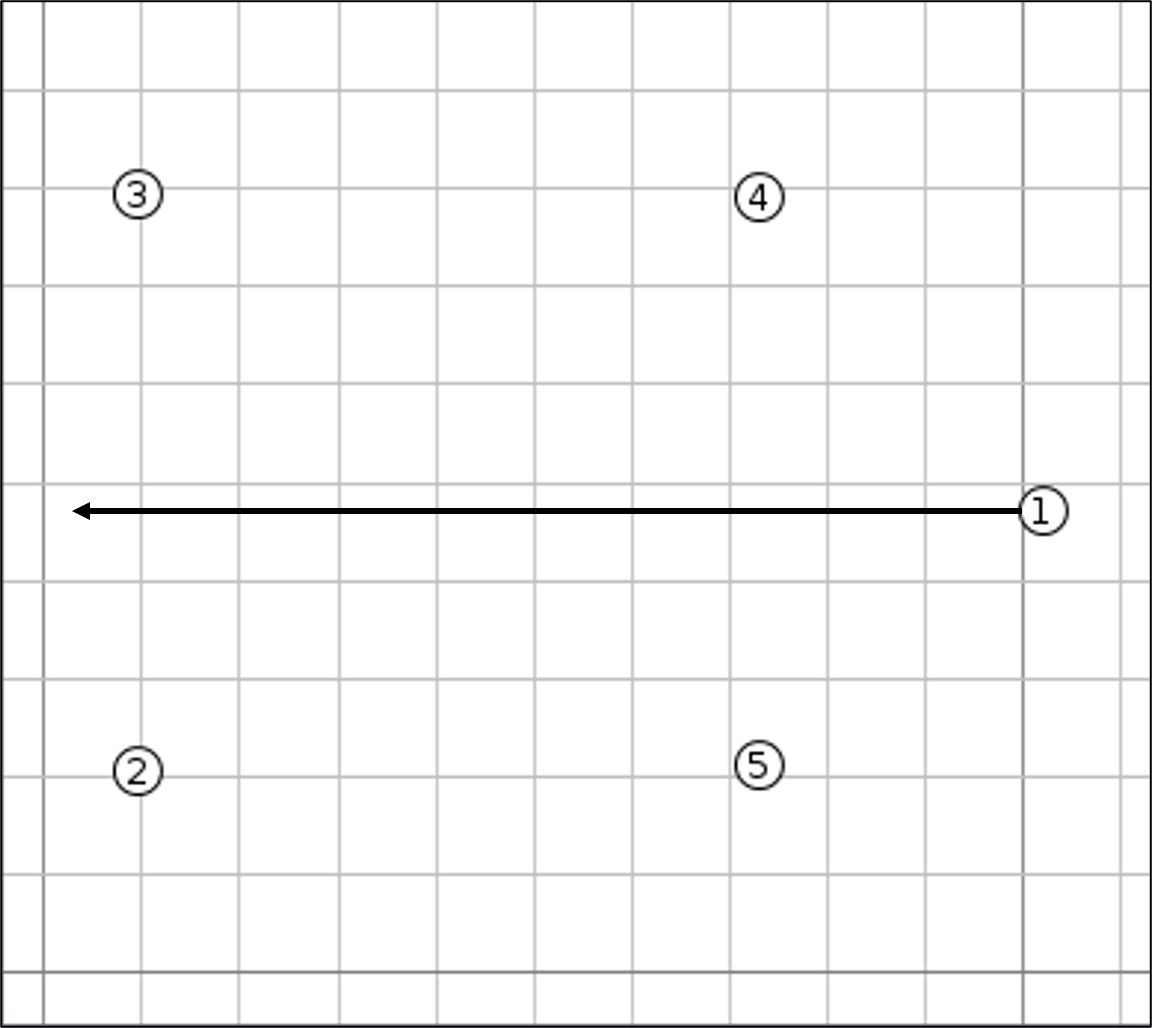
\includegraphics[cfbox=black 1pt 1pt,scale=0.21]{./simulation2.png}
        \subcaption{Crossing aisle}
    \end{minipage}\hspace{10pt}
     \begin{minipage}[c]{.3\linewidth}
        \centering
        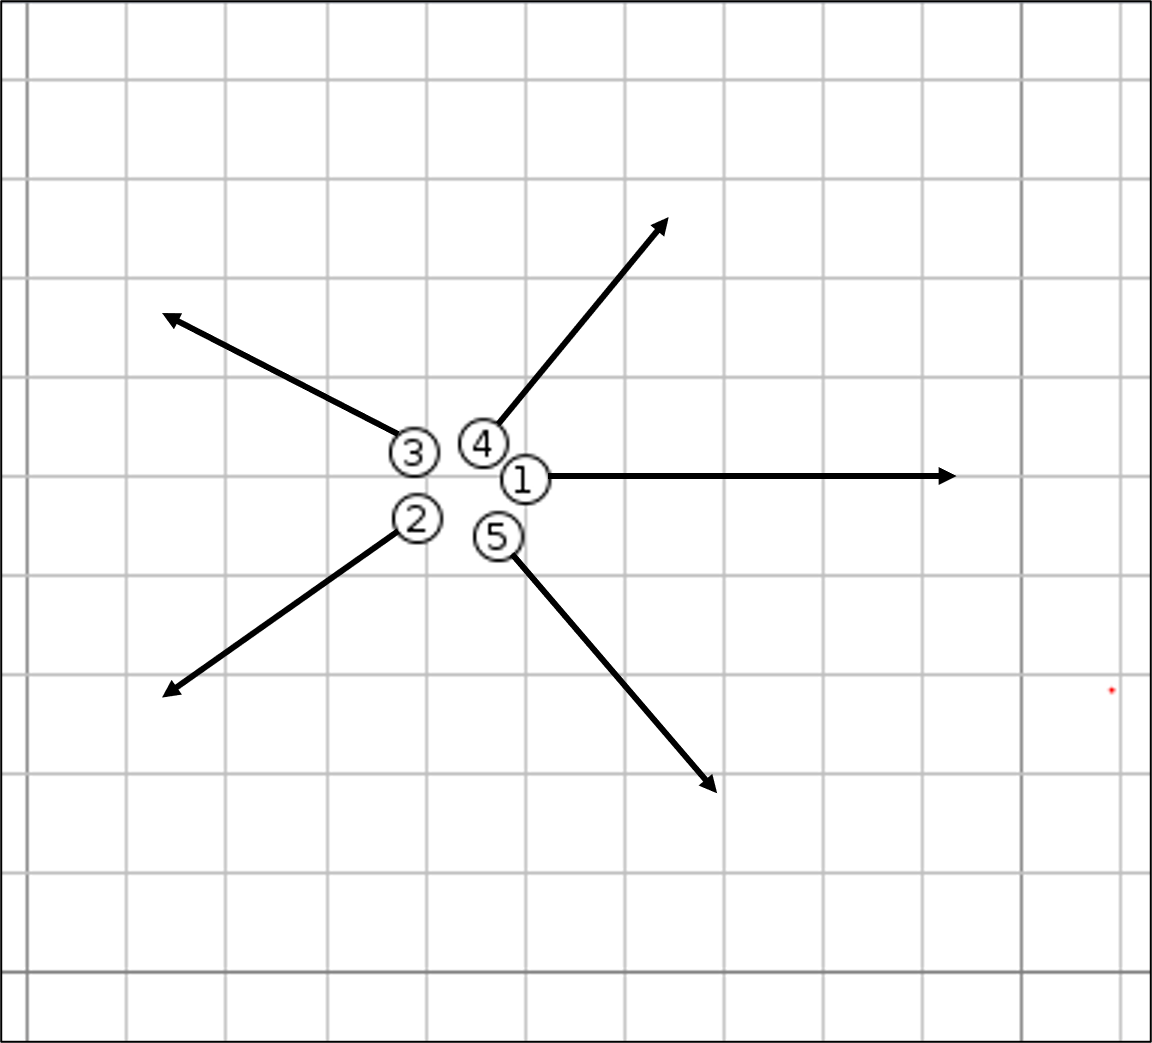
\includegraphics[cfbox=black 1pt 1pt,scale=0.21]{./simulation3.png}
        \subcaption{Moving away from center}
    \end{minipage}\hspace{10pt}
    \begin{minipage}[c]{.3\linewidth}
        \centering
        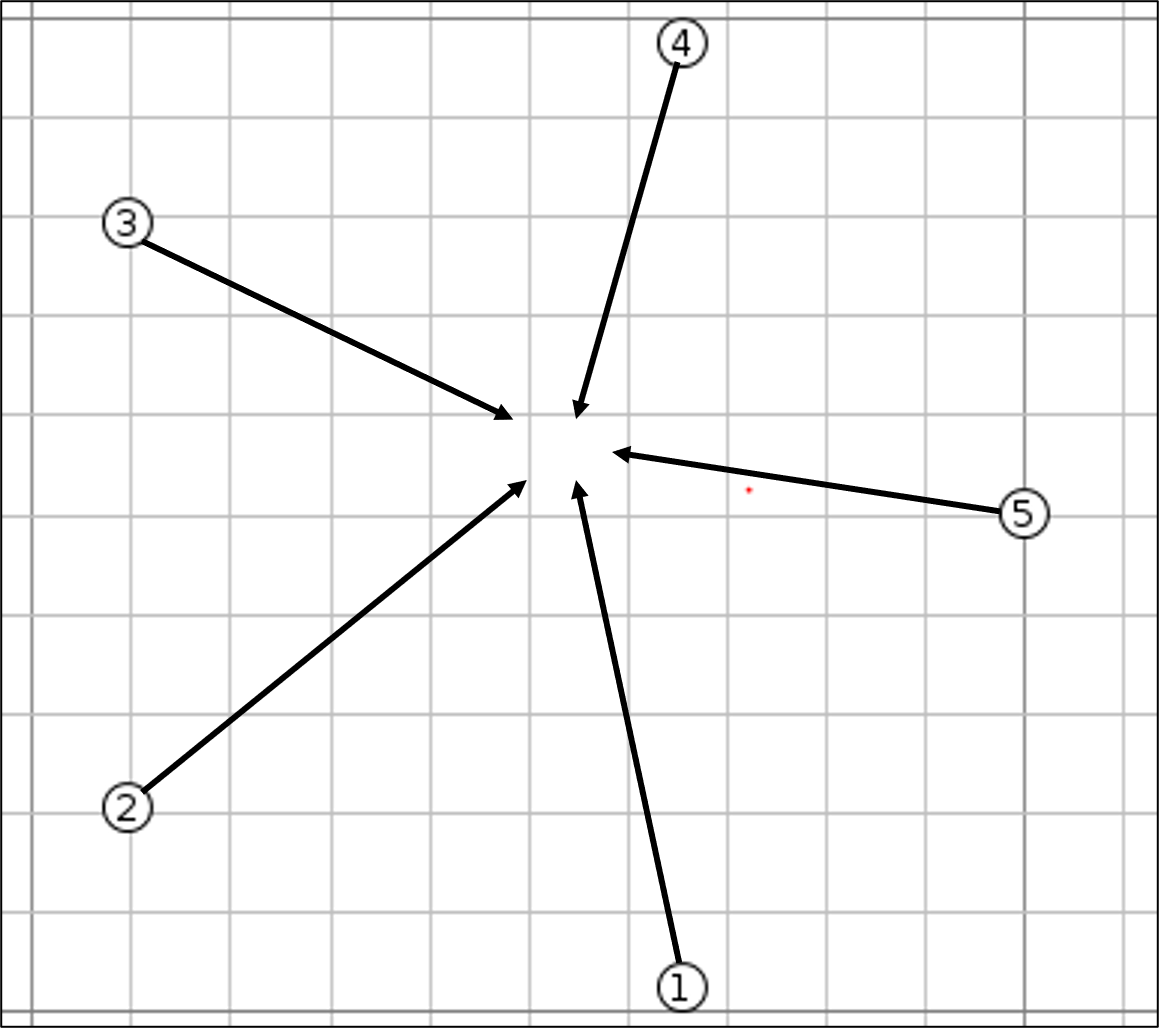
\includegraphics[cfbox=black 1pt 1pt,scale=0.21]{./simulation1.png}
        \subcaption{collapsing in one point}
    \end{minipage}
    \caption{Simulations representation.}
    \label{fig:simulationFIG}
\end{figure}

\section{Warnings}
Since IFTTT impose a limit on the triggerable events per minute\footnote{IFTTT limit: 120 events/minute}, in the node red part a rate limit is necessary. to better appreciate the simulation results a speed limit in the Cooja simulator is recommended



\pagebreak
\pagebreak
\clearpage
\end{document}